\documentclass[final]{beamer}
\mode<presentation>
{
        \usetheme{SU}
}
\usepackage{graphicx}
\usepackage[english]{babel}
\usepackage[utf8]{inputenc}
\usepackage[orientation=portrait,size=a1,scale=1.4]{beamerposter}
\usepackage{tikz-dependency}

\usepackage[T1, OT1]{fontenc}
\DeclareTextSymbolDefault{\dh}{T1}

\title{Universal Dependencies \\ for Swedish Sign Language}
\author{Robert {\"O}stling, Carl B{\"o}rstell, Moa G{\"a}rdenfors,
    Mats Wir{\'e}n}
\institute{Stockholm University}

\begin{document}

\addtobeamertemplate{headline}{} 
{
    \begin{tikzpicture}[remember picture,overlay] 
        \node [shift={(-5cm,-3cm)}] at (current page.north east)
        {
\includegraphics[height=5cm]{logo-neg-engelsk_rgb.eps}}; 
    \end{tikzpicture} 
}

\begin{frame}{}
    \vfill
    \begin{columns}[t]
        \begin{column}{.48\linewidth}

            \begin{block}{\large Swedish Sign Language (SSL)}
                \begin{itemize}
                    \item Used by $\approx$ 10,000 as a primary language
                    \item Documented history of 200 years
                    \item Official status since 1981
                \end{itemize}
            \end{block}

            \begin{block}{\large Existing computer resources}
                \begin{itemize}
                    \item Swedish Sign Language Corpus (SSLC)
                    \item Swedish Sign Language Dictionary (SSLD)
                    \item (\textbf{NEW!}) Universal Dependencies treebank
                \end{itemize}
            \end{block}

            \begin{block}{\large Universal Dependencies (UD)}
                \begin{itemize}
                    \item Language-independent(ish) annotation standard
                    \item 70 treebanks in 50 languages
                    \item 49 spoken/written, (\textbf{NEW!}) 1 signed
                    \item 2 with transcribed conversation (Slovene, SSL)
                \end{itemize}
            \end{block}

            \begin{block}{\large Challenges}
                \begin{itemize}
                    \item The two hands may produce different signs
                        simultaneously: no fixed linear order
                    \item Little previous work and grammatical traditions
                    \item Also an opportunity, from the UD point of view
                    \item How should the UD standard or parsing algorithms be
                        adapted to better handle sign languages?
                \end{itemize}
            \end{block}


        \end{column}

        \begin{column}{.48\linewidth}

            \begin{block}{\large The SSL Treebank}
                \begin{itemize}
                    \item A first step: 672 tokens in UD 1.4
                    \item Annotation work continues
                    \item The first dependency treebank of a sign language
                \end{itemize}
            \end{block}

           \begin{center}
            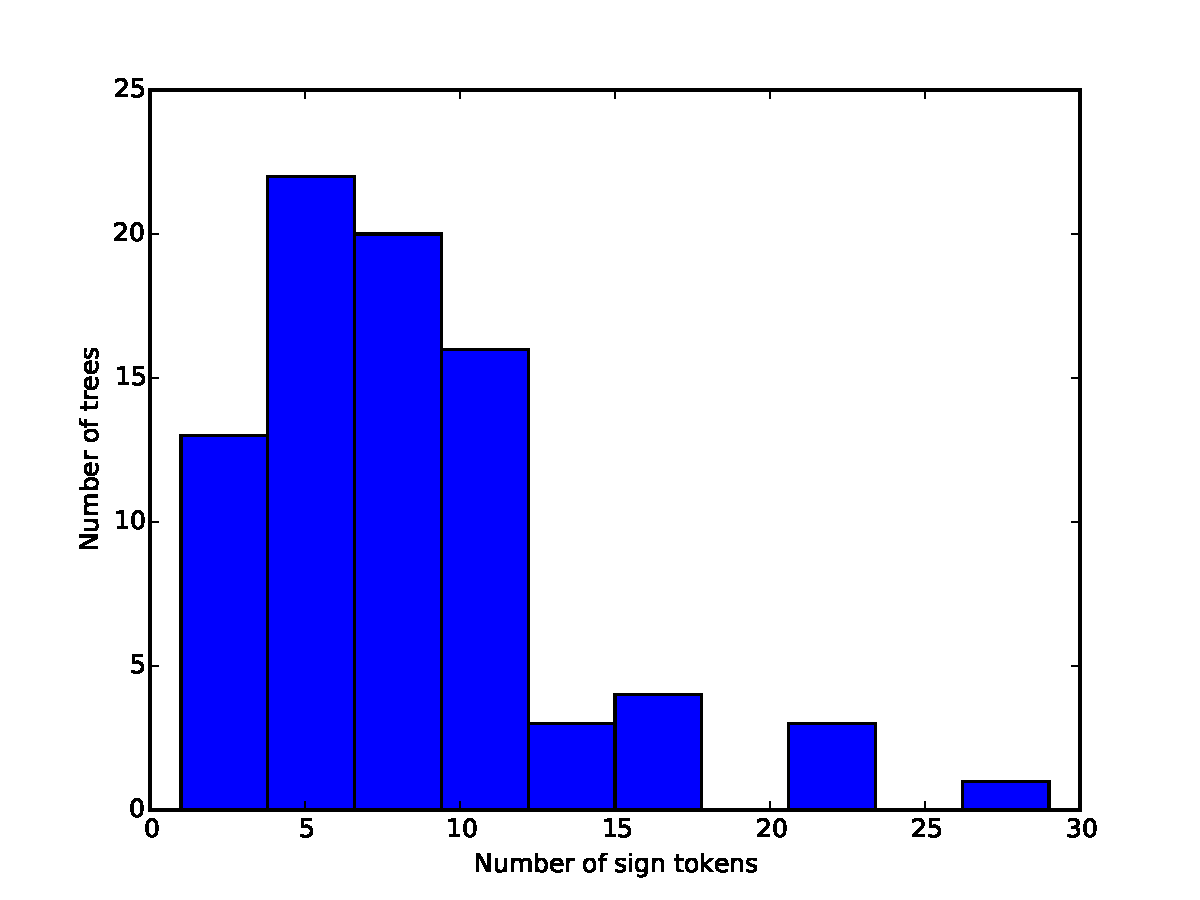
\includegraphics[width=1.0\linewidth]{../nodalida2017/treesizes.pdf}
           \end{center}

            \begin{block}{\large Parseable?}
                \begin{itemize}
                    \item 28 LAS (36 UAS) on the test set
                    \item 334 \emph{tokens} of training data is not enough for
                        serious parsing
                \end{itemize}
            \end{block}

            %\begin{block}{\large Questions opened}
            %    \begin{itemize}
            %        %\item What is the sound of a tree falling where no one
            %        %    hears it, or of one hand clapping?
            %        %\item (\textbf{NEW!}) What is the projectivity status of
            %        %    a tree containing overlapping signs from two hands?
            %        \item How can the UD formalism be better adapted to sign
            %            languages?
            %        \item How do parsing algorithms need to be adapted?
            %    \end{itemize}
            %\end{block}

          \end{column}
        \end{columns}
    %\begin{block}{\Large Conclusions}
    %    \Large
    %\end{block}
           \begin{center}

\vspace{2cm}
\begin{dependency}[theme = simple, edge style={very thick}, label style={scale=1.2}]
   \begin{deptext}[column sep=1em]
      \texttt{verb} \& \texttt{verb} \& \texttt{verb} \& \texttt{noun} \& \texttt{det} \& \texttt{verb} \\
      \textsc{s{\"a}tta-sig} \& \textsc{{\"a}ta}(Q) \& \textsc{titta-p{\aa}} \& \textsc{sn{\"o}{\string^}gubbe} \& \textsc{pek} \& \textsc{{\"a}ta}(Q) \\
      \textsc{sit-down} \& \textsc{eat}(Q) \& \textsc{look-at} \& \textsc{snow{\string^}old-man} \& \textsc{point} \& \textsc{eat}(Q) \\
   \end{deptext}
   \deproot{1}{root}
   \depedge{1}{2}{conj}
   \depedge{1}{3}{conj}
   \depedge{3}{4}{dobj}
   \depedge{4}{5}{det}
   \depedge[arc angle=50]{2}{6}{conj}
   \node (translation) [below left of = \wordref{1}{1}, xshift=12cm, yshift=-3em] {
   `He is sitting there eating looking out at
   the snowman.'};
\end{dependency}
           \end{center}
      \end{frame}
    \end{document}

